\providecommand{\main}{../../../..}
\documentclass[\main/dresen_thesis.tex]{subfiles}

\begin{document}
  \label{sec:looselyPackedNS:nanoparticle:tem}
  \begin{figure}[!htbp]
    \centering
    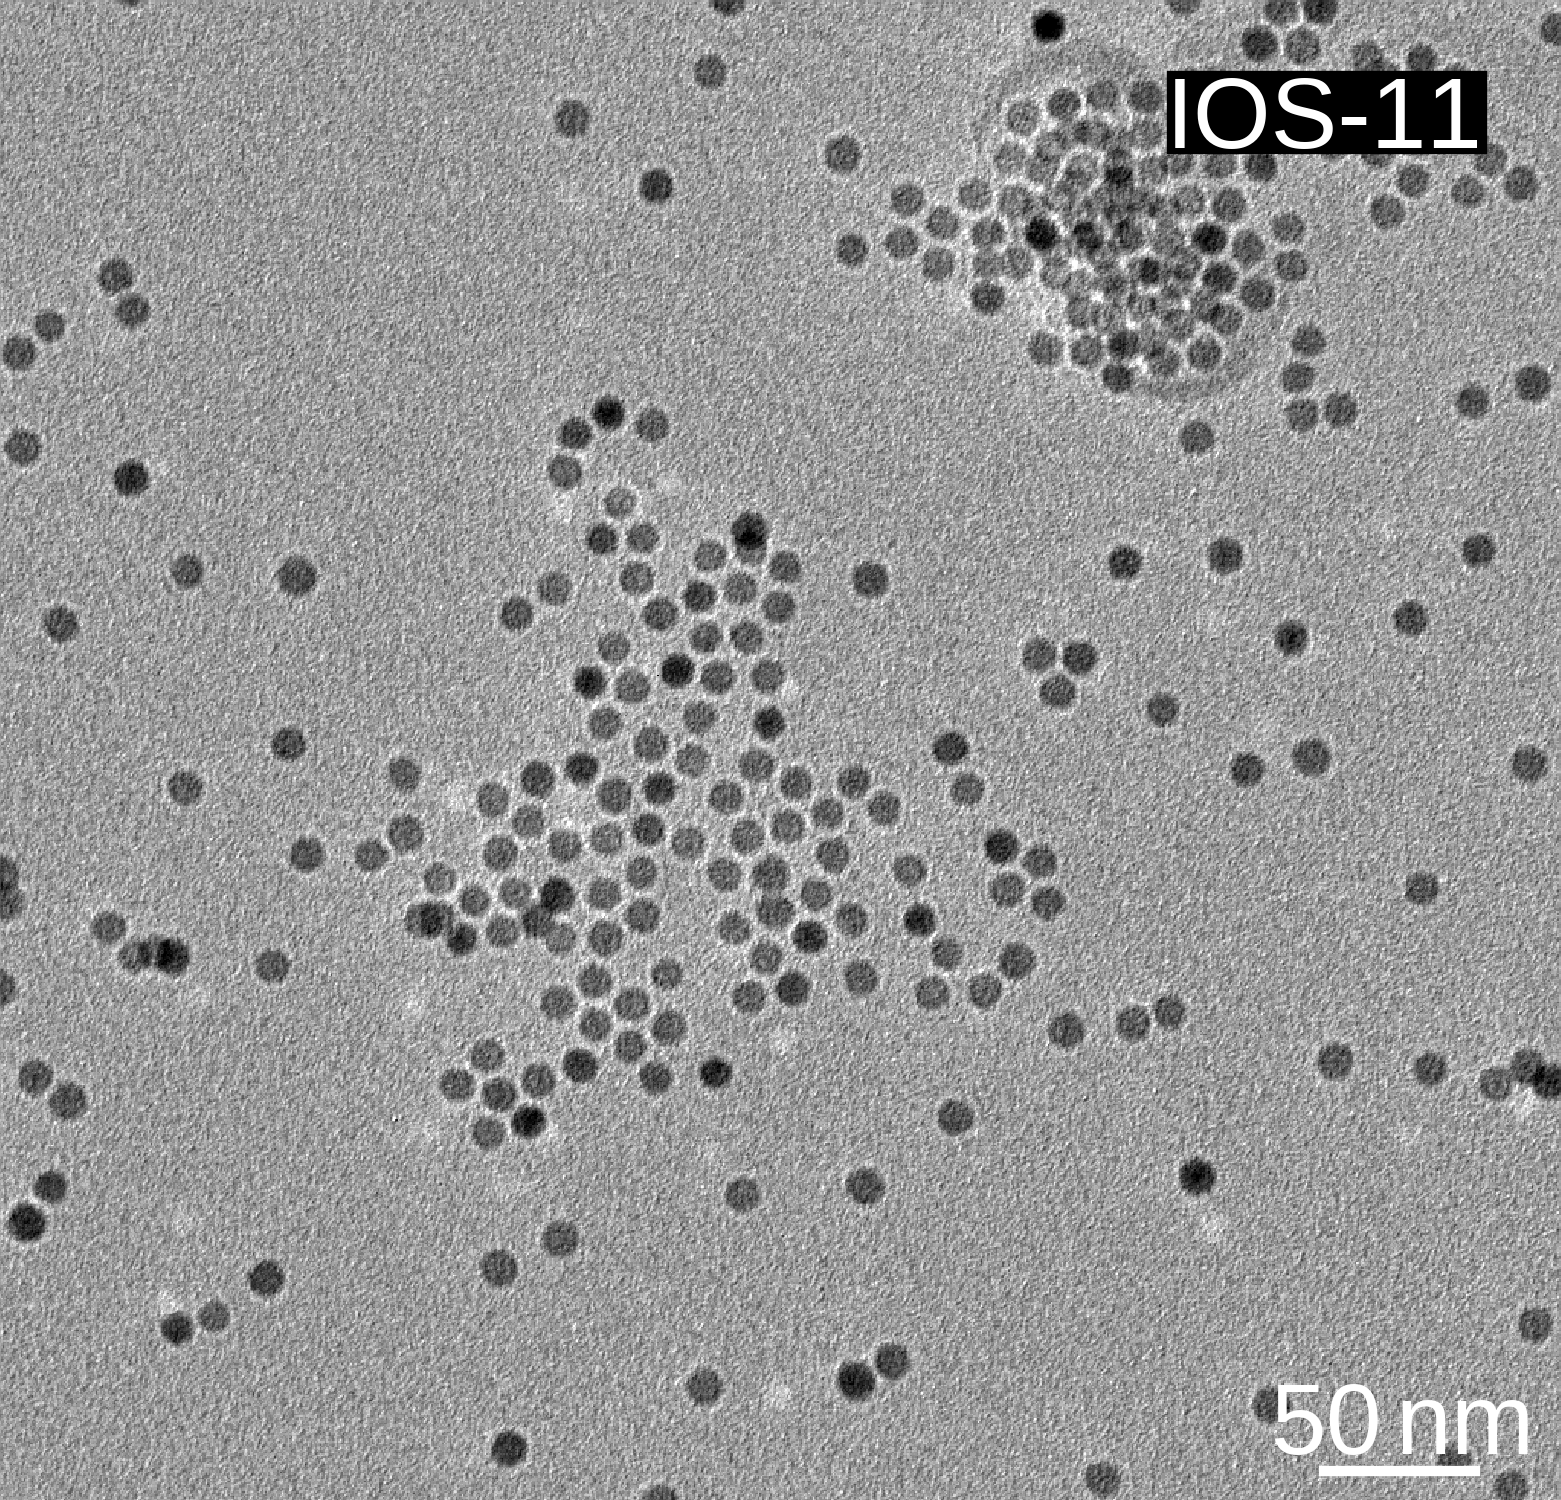
\includegraphics{looselyPackedNP_TEM_IOS-11}
    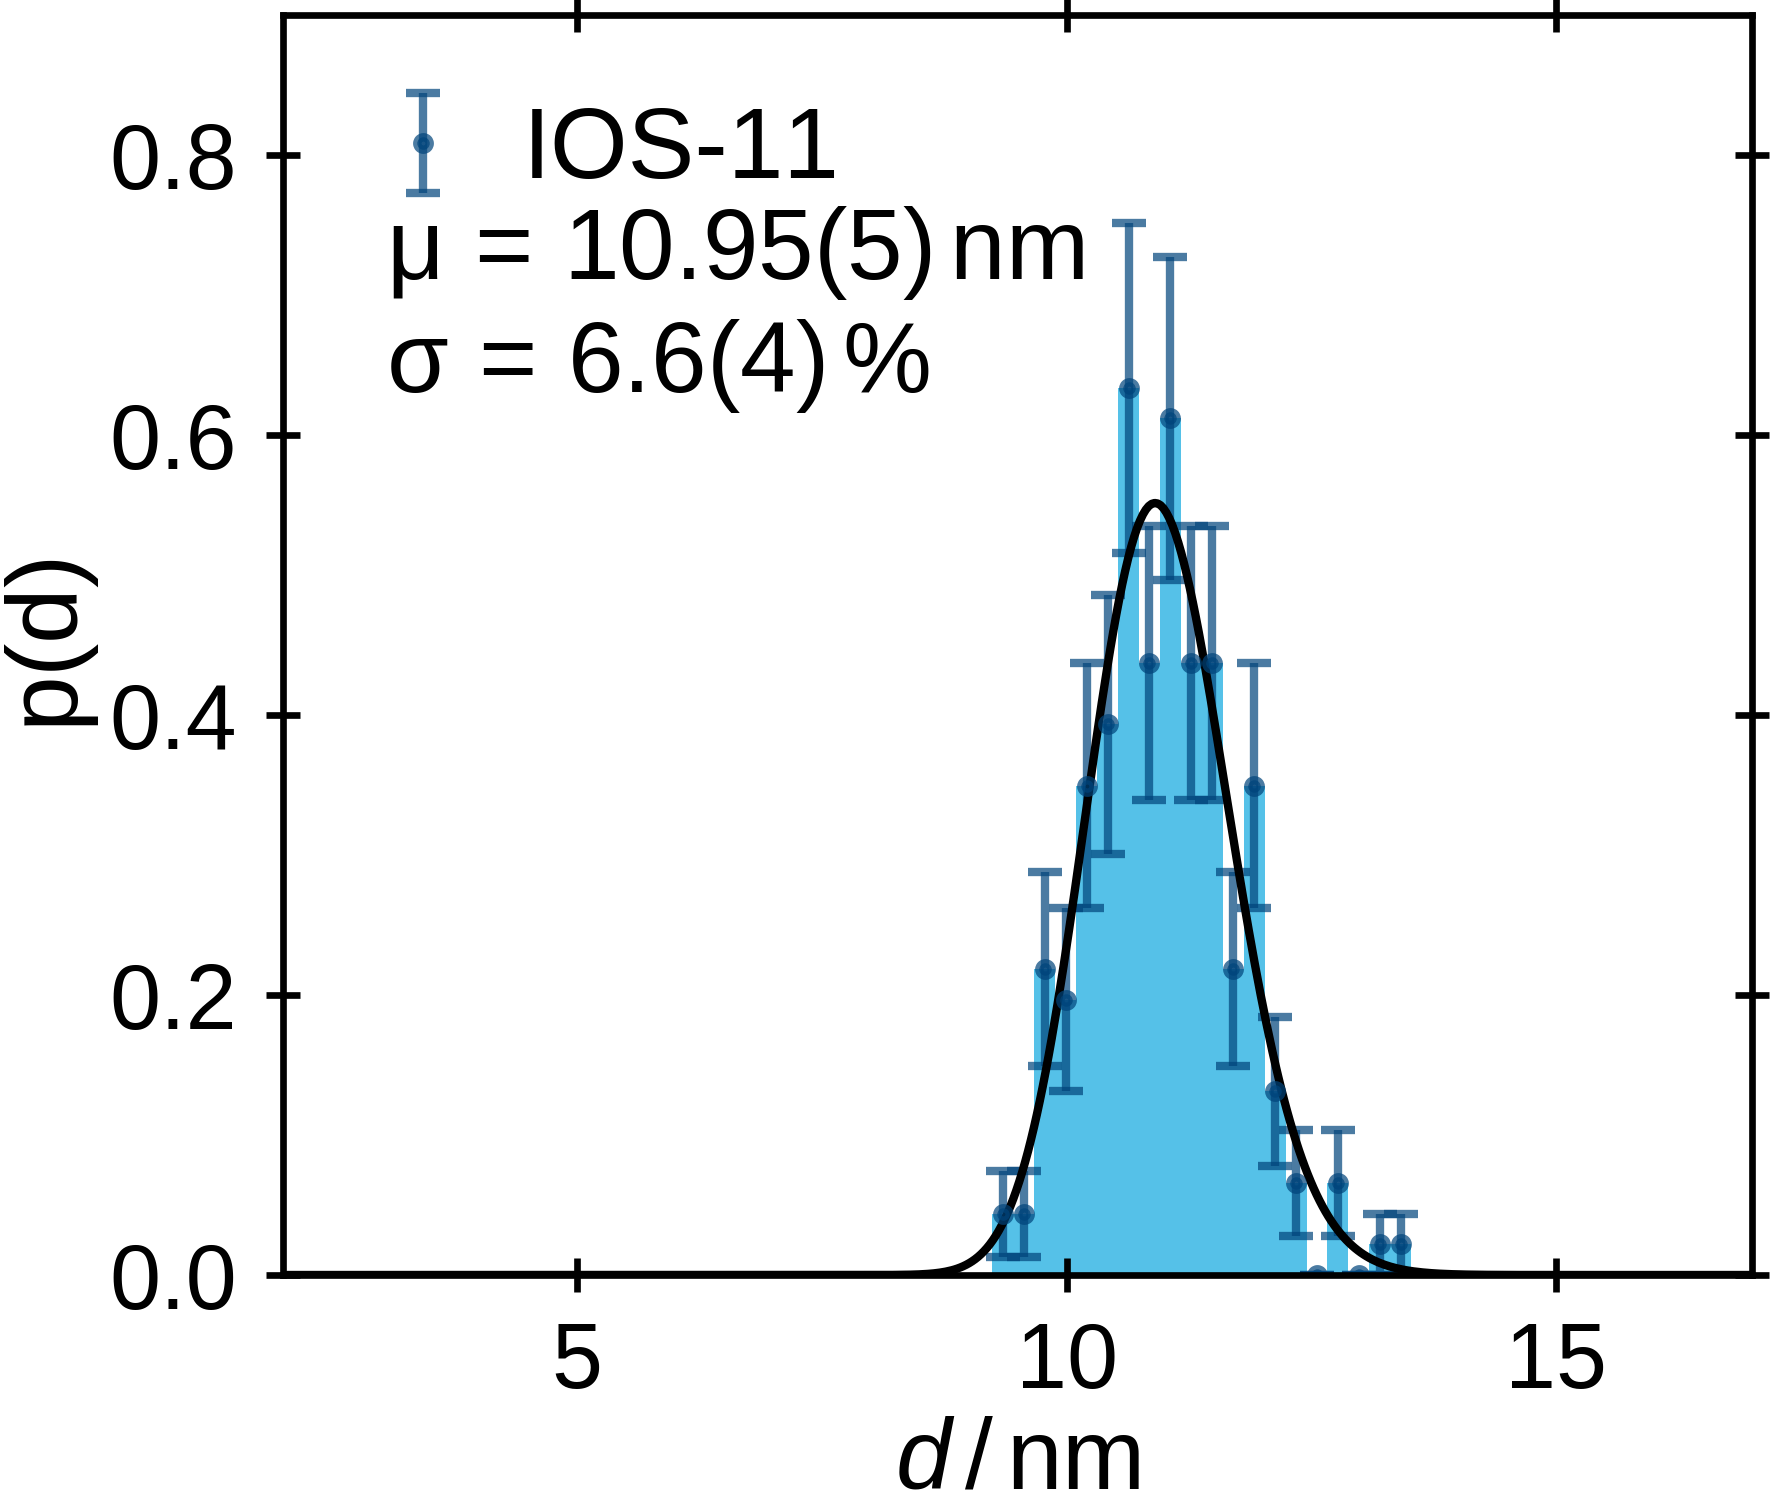
\includegraphics{looselyPackedNP_TEM_IOS-11_sizeDist}
    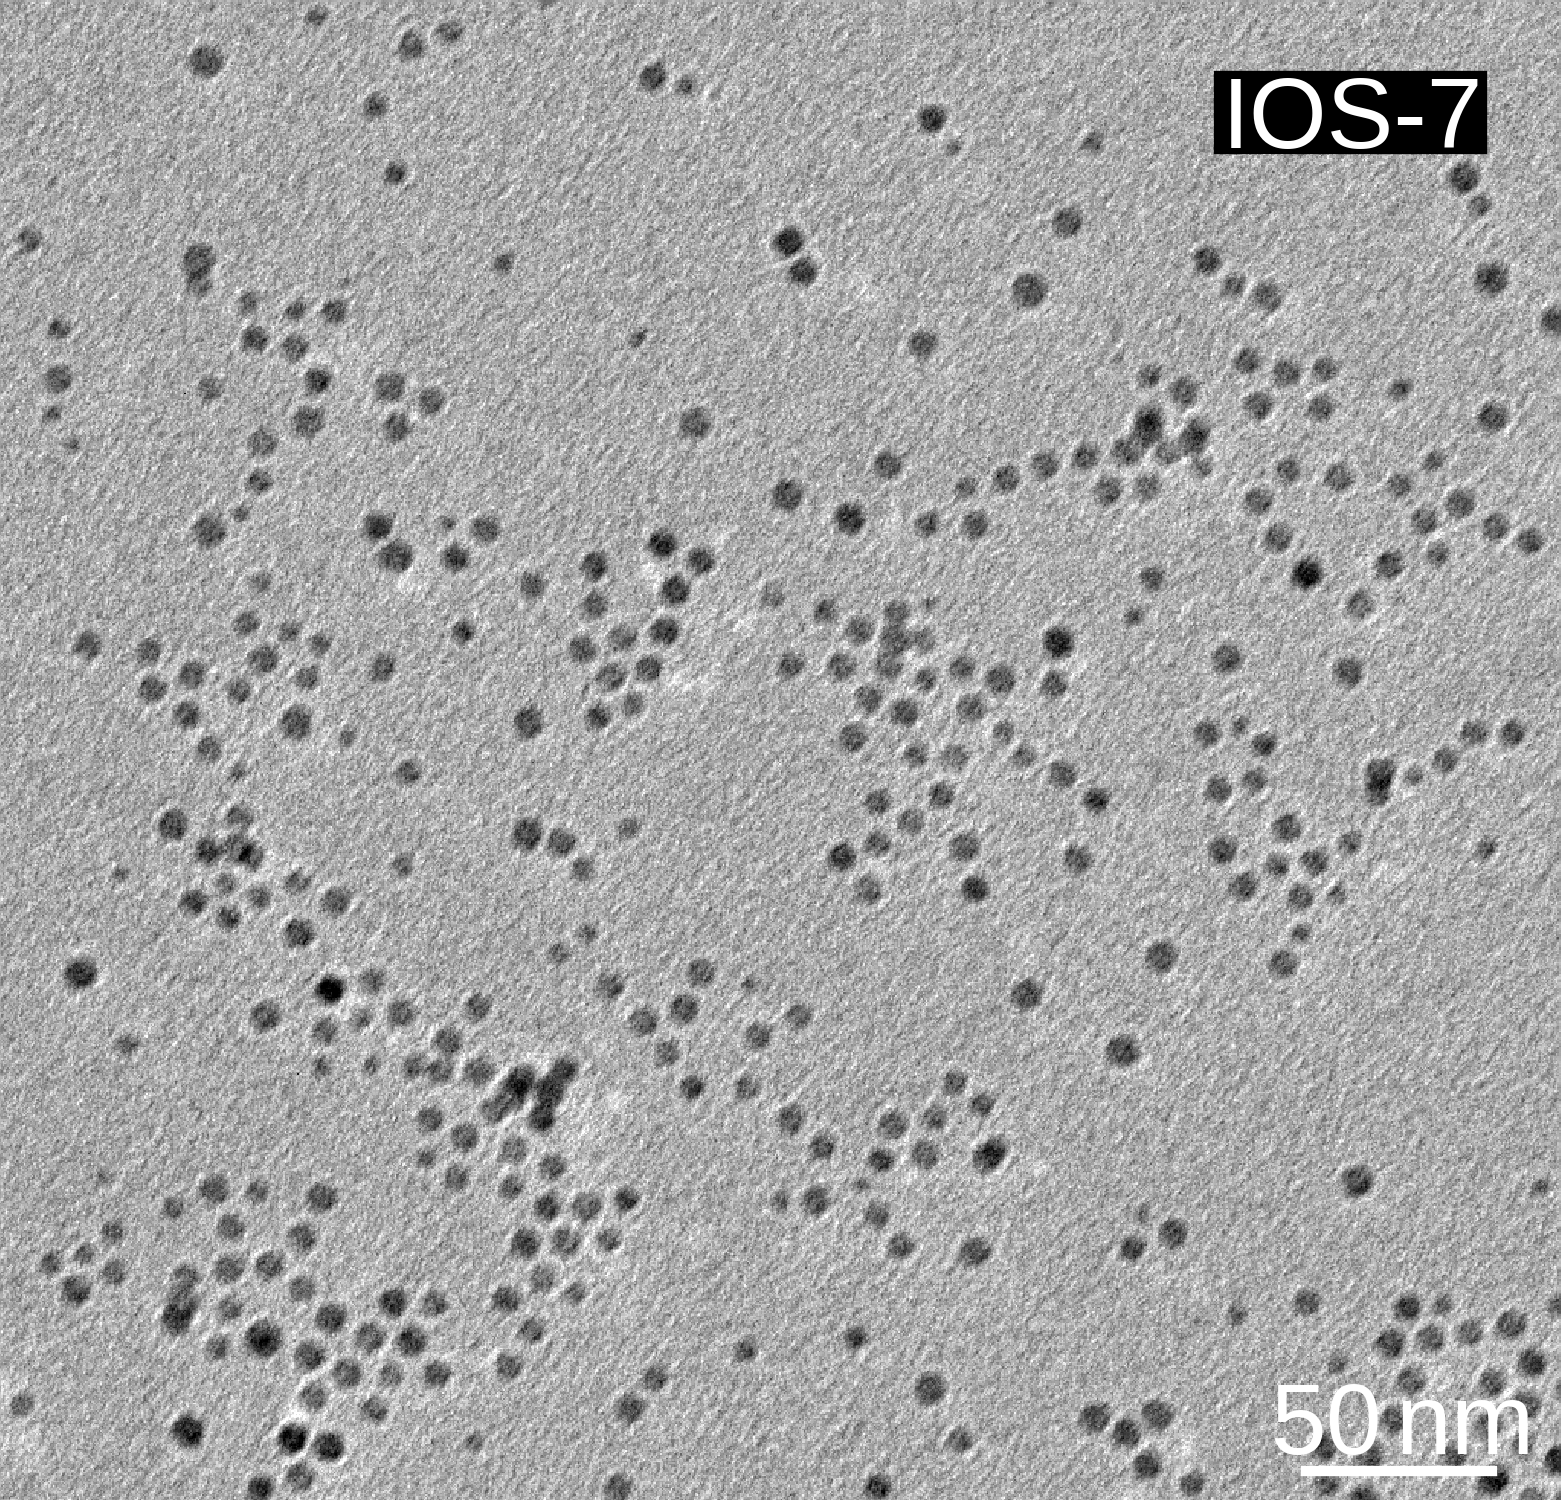
\includegraphics{looselyPackedNP_TEM_IOS-7}
    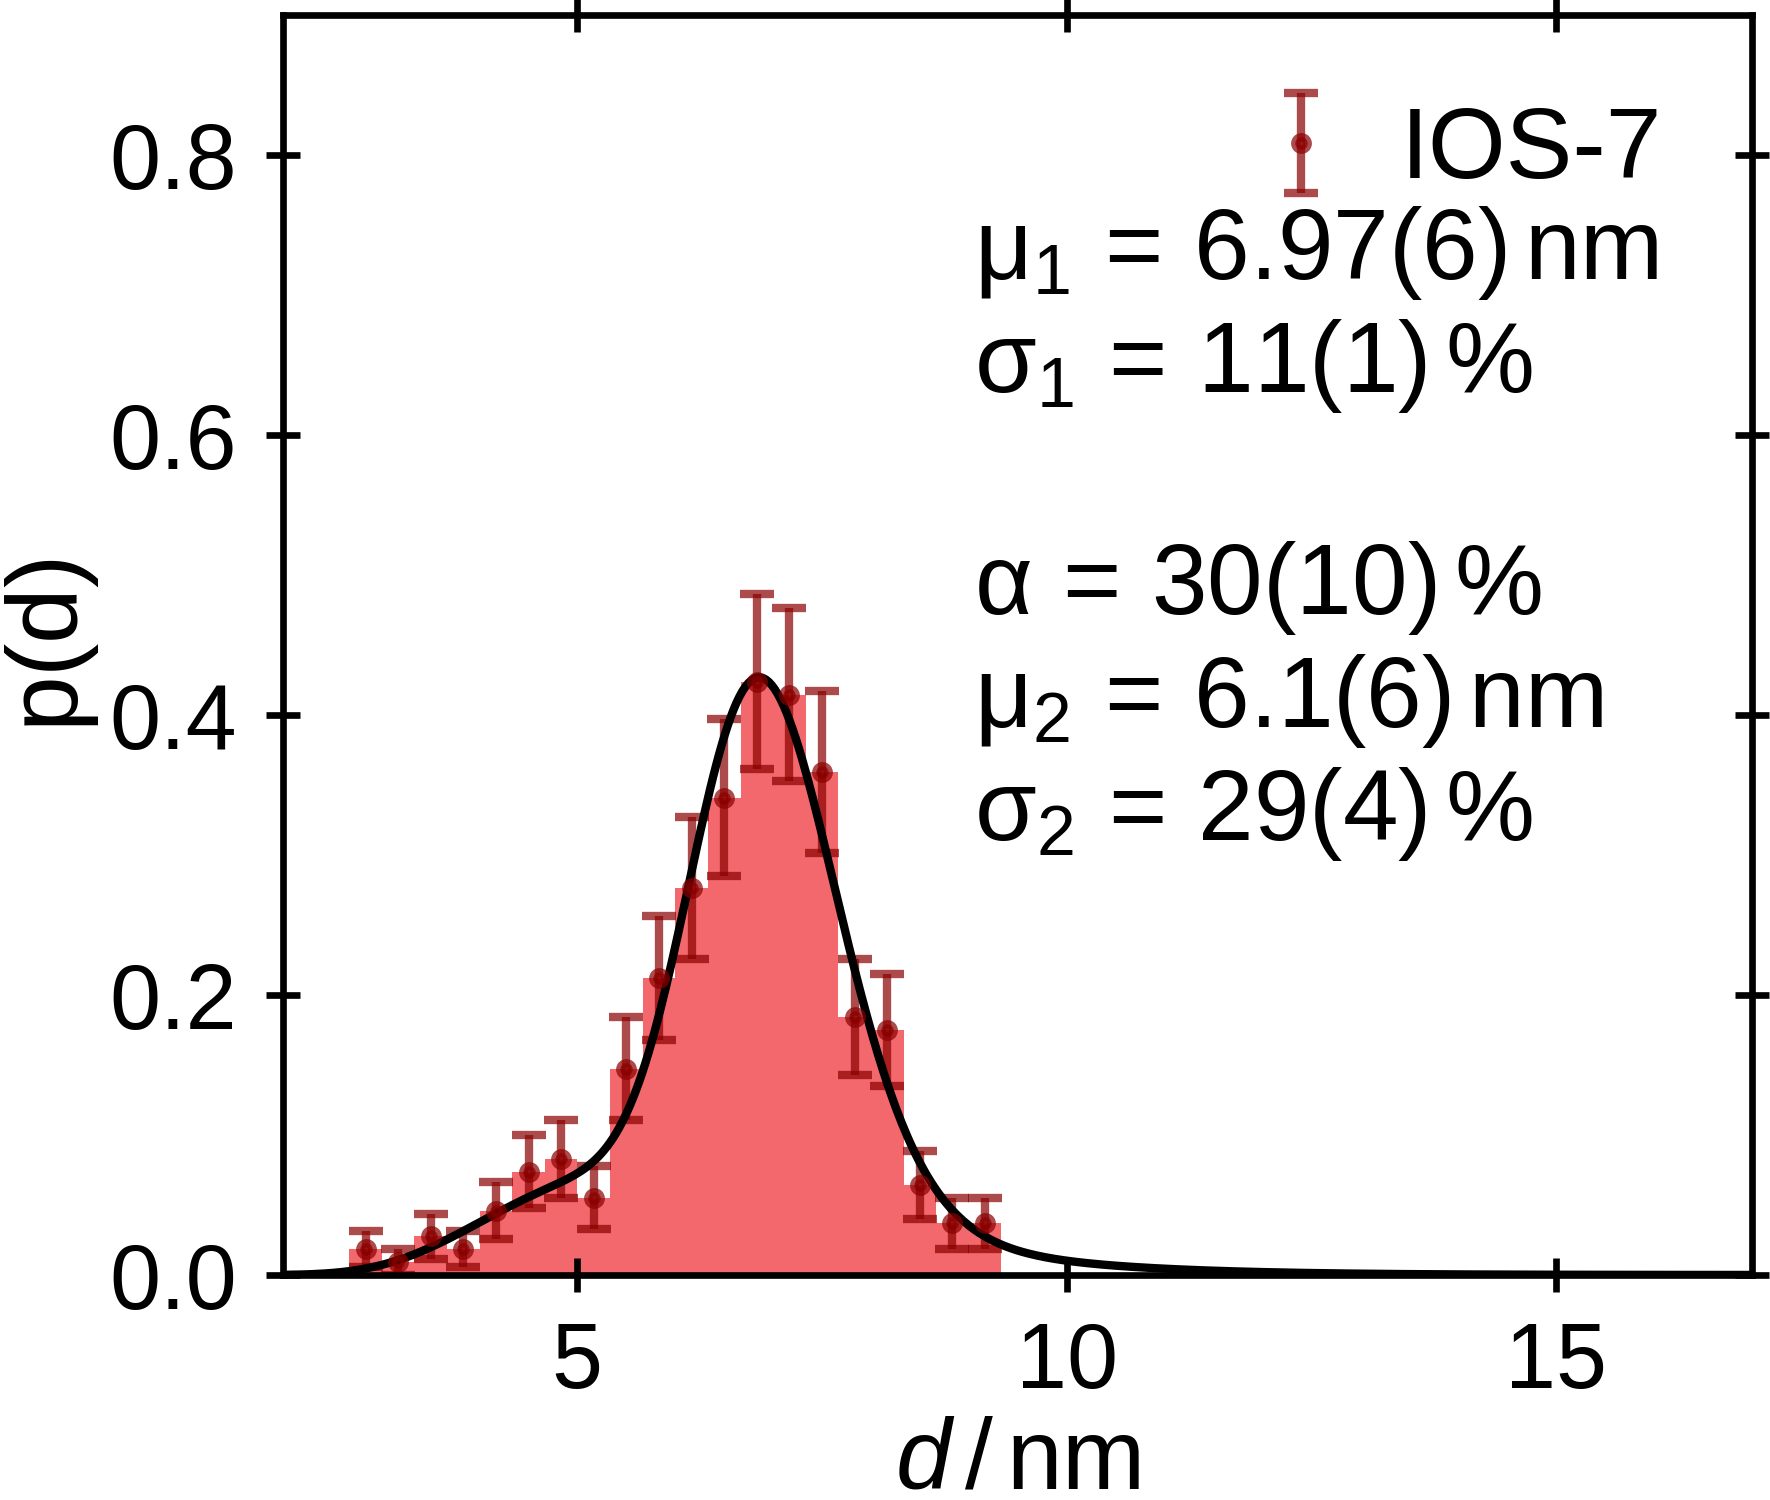
\includegraphics{looselyPackedNP_TEM_IOS-7_sizeDist}
    \caption{\label{fig:looselyPackedNP:nanoparticle:tem}TEM micrographs (left) and the particle size distribution of the diameter (right) for the iron oxide nanospheres IOS-11 (upper) and IOS-7 (lower).}
  \end{figure}

  Exemplarly micrographs of the two iron oxide nanosphere batches and the histograms of the counted occurence of diameters are shown in \reffig{fig:looselyPackedNP:nanoparticle:tem}.
  The spherical shape can be confirmed for both batches, where IOS-11 qualitatively shows a greater size and smaller size distribution in direct comparison to IOS-7.
  The different size is confirmed in the histograms and the fit to log-normal size distributions, where IOS-11 has a mean diameter of $10.95(5) \unit{nm}$ with a distribution of $6.6(4) \%$. 
  The batch IOS-7 can not be fully described by a single log-normal distribution and needs a bimodal fit, where one fraction has a mean diameter of $6.97(6) \unit{nm}$ with $11(1) \%$ size distribution and the second mode of nanoparticles has a mean diameter of $6.0(6) \unit{nm}$ and a size distribution of $29(4) \%$.
  The fraction of the mode with the broader size distribution is estimated to be $30(10) \%$ of the sample.

  \begin{table}[!htbp]
    \centering
    \caption{\label{tab:looselyPackedNP:nanoparticle:temModel}Parameters estimated for the size distribution of IOS-11 and IOS-7 from fitting a (bimodal) log-normal size distribution.}
    \begin{tabular}{ c | l | l }
      \textbf{TEM}  & IOS-11 & IOS-7 \\
      \hline
      $\mu_1$     & $10.95(5) \unit{nm}$  & $6.97(6) \unit{nm}$ \\
      $\sigma_1$  & $6.6(4) \unit{\%}$    & $11(1) \unit{\%}$ \\
      $1 - \alpha$&                       & $30(10)  \unit{\%}$   \\
      $\mu_2$     &                       & $6.0(6) \unit{nm}$ \\
      $\sigma_2$  &                       & $29(4) \unit{\%}$ \\
      \hline
    \end{tabular}
  \end{table}
\end{document}